\overlays{4}{
\begin{slide}{Com'è questo Linux?}
\onlySlide*{1} {
{\tiny
{\black
GNU/Linux può essere visto in molte forme diverse. Quasi tutte seguono
delle linee di principio simili, ma in genere ognuna ha una
particolarità, ognuna è stata creata per fare qualcosa di particolare.

Possiamo dire, ognuna ha un obiettivo ben precisa.

Sebbene il sistema operativo Windows, purtroppo enormemente più diffuso
di GNU/Linux, abbia {\bfseries un} solo modo di gestire il desktop,
GNU/Linux da all'utente la possibilità di gestire autonomamente, e di
{\bfseries decidere} come gestire il proprio desktop.

Ci sono ambienti come KDE o Gnome che tendono ad essere completi ed a
gestire ogni aspetto dell'uso del computer: dal movimento del mouse allo
scaricamento della posta, passando per la gestione dei files e delle
cartelle, delle connessioni di rete e delle risorse del computer.

Ci sono ambienti invece dove tutto il resto viene lasciato all'utente,
che può farlo a mano oppure predisporre altri programmi per farlo.
Questi ambienti hanno lo svantaggio, di essere più difficili da usare 
e più lunghi da imparare ad usare. Danno però una possibilità di 
personalizzazione quasi totale.

Queste slides sono state create sotto uno di questi: 
\href{http://www.nongnu.org/ratpoison/}{Ratpoison}.
}
}
}


\onlySlide*{2} {
Questo ad esempio è KDE, versione 3.5.10

\flushright{
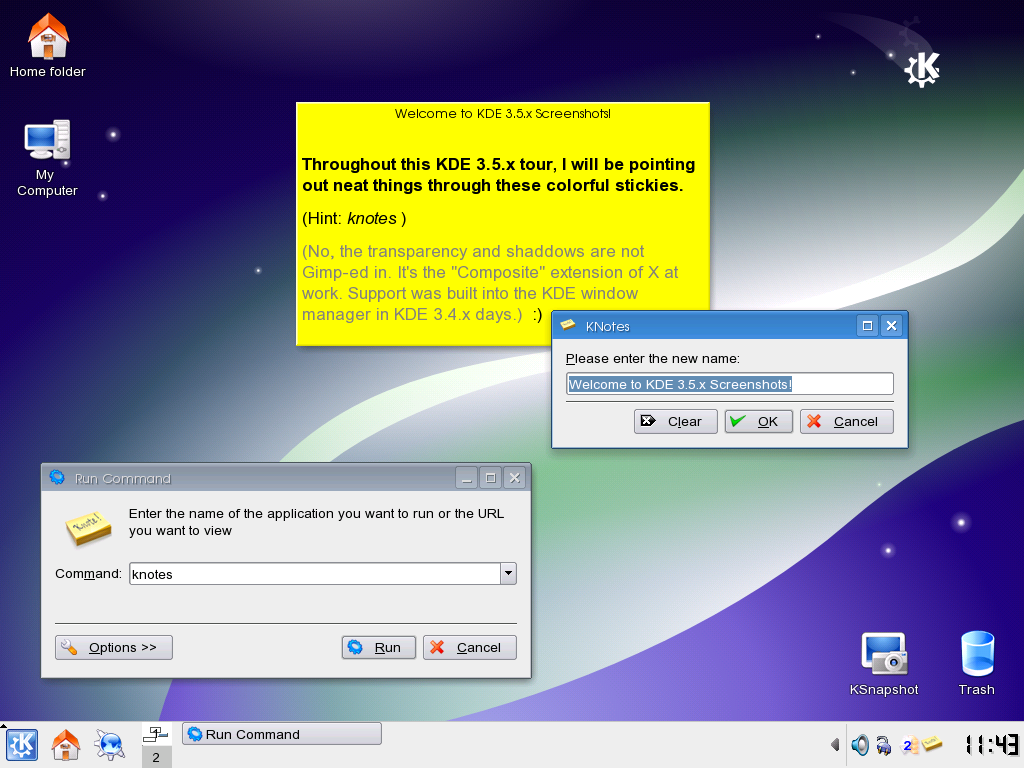
\includegraphics[width=8cm,height=6cm]{immagini/kde.eps}
}
}


\onlySlide*{3} {
Gnome 2.24:

\flushright{
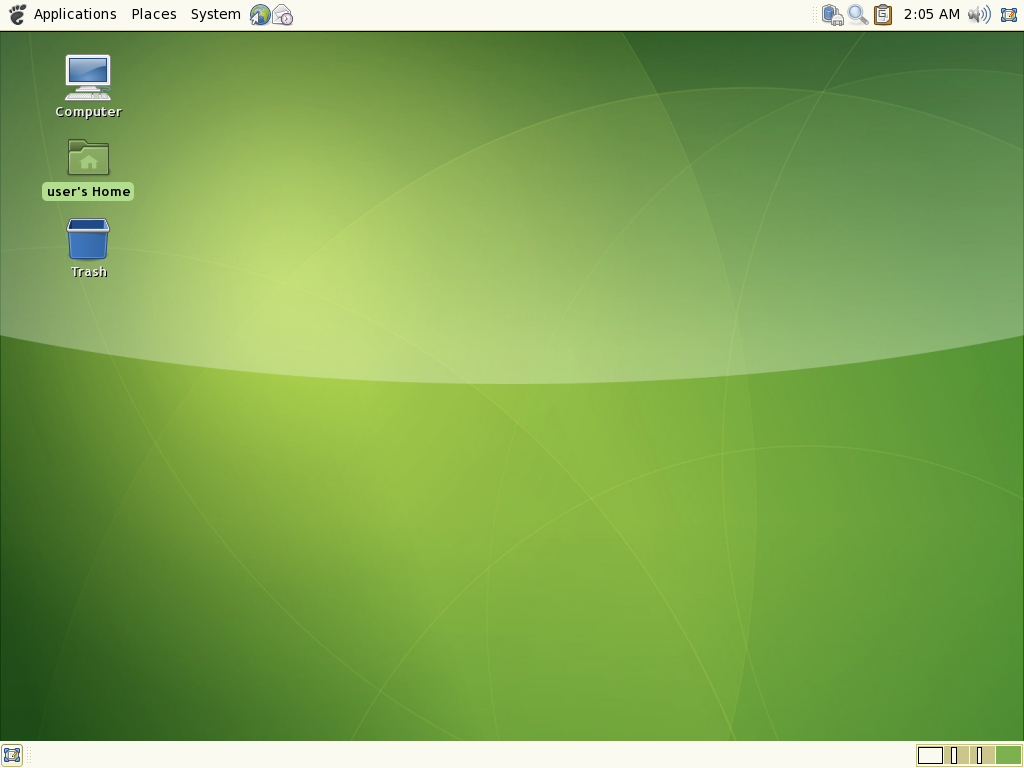
\includegraphics[width=8cm,height=6cm]{immagini/gnome.eps}
}
}


\onlySlide*{4} {
Questo invece è Ratpoison.
\flushright{
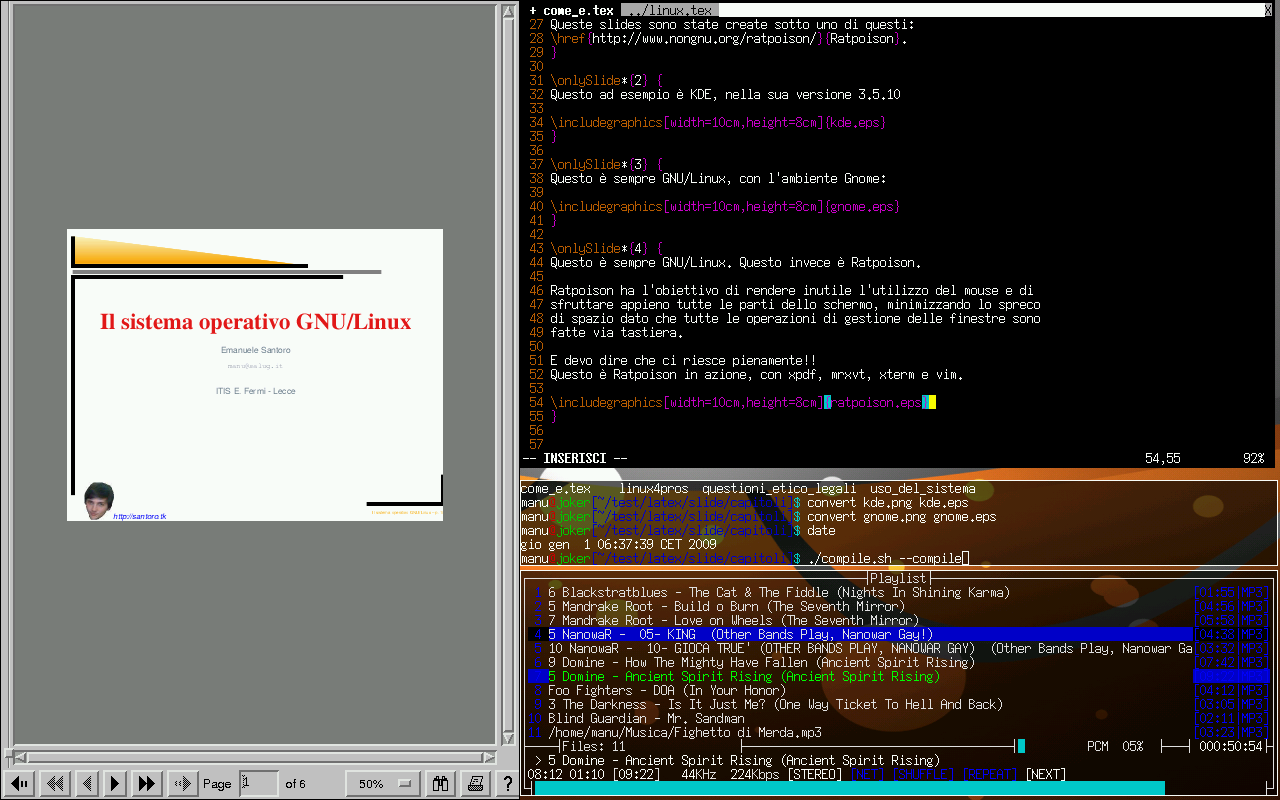
\includegraphics[width=10cm,height=6cm]{immagini/ratpoison.eps}
}
}



\end{slide}}
